\section{Interpretation of Results}
\label{sec:InterpretationOfResults}
%Try to give an interpretation of you results in your answers to the problems.
%Compare results with closed form solution
It can be shown by inserting into \eqref{eq:Nature1} that 
\begin{align}
	u(x) = 1-(1-e^{-10})x-e^{-10x}
	\label{eq:IntOfResult1a}
\end{align}
is a solution to the differential equation for $p(x)=100e^{-10x}$ and hence $f(x)=100e^{-10x} h^2$. 
The expression in \eqref{eq:IntOfResult1a} is the closed-form solution to the one-dimensional Poisson equation.

In the figure below the closed-form solution given in \eqref{eq:IntOfResult1a} is plotted as a function of $x$ together with the numerical solution gained from the algorithm described in \secref{sec:DescriptionOfTheAlgorithm} for three different number of grid points $n$, namely 10, 100 and 1,000.  
The plots are made in MatLab and the closed-form solution is plotted with 1000 grid points. 
The source code for the MatLab plot can be seen in \appref{app:MatLabSolution}.
\begin{figure}[H]
	\centering
	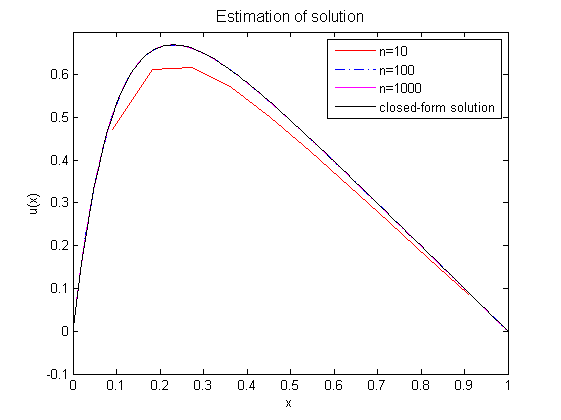
\includegraphics[width=0.75\textwidth]{Figures/estimaition_of_solution.png}
	\caption{Plot of the closed-form solution together with the numerical solution for different number of grid points. It is evident that the accuracy of the numerical solution gets better when number of grid points is increased from $n=10$ to $n=100$ and $n=1000$.}
	\label{fig:IntOfResult1}
\end{figure}
From \figref{fig:IntOfResult1} it is easily seen that by increasing the number of grid points from $n=10$ to $n=100$ the precision of the solution is better. 
%However, it is not evident from the figure that a further increment of $n$ improves the precision further. 
By zooming in on the figure, it can be seen that an increment of $n$ from 100 to 1000 actually gives a further improvement to the numerical solution, as can be seen in \figref{fig:IntOfResult2}.   
\begin{figure}[H]
	\centering
	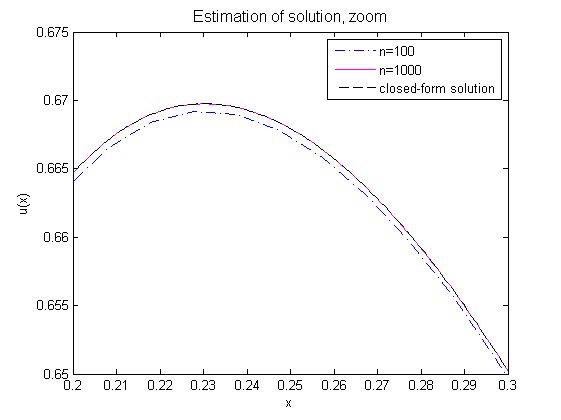
\includegraphics[width=0.75\textwidth]{Figures/estimaition_of_solution_zoom.png}
	\caption{Zoom of \figref{fig:IntOfResult1}. It is seen that a further increment of $n$ from 100 to 1000 actually improves the accuracy of the result.}
	\label{fig:IntOfResult2}
\end{figure}

%Data for relative error (data in excel sheed) gained from the cpp code
From \figref{fig:IntOfResult1} and \figref{fig:IntOfResult2} it is evident that there is a deviation between the closed-form solution $\v{u}$ and the numerical solution gained by the algorithm made in the project, and that the deviation decreases with increasing number of investigated grid points $n$.
To see how this deviation actually reacts on a change in number of grid points, which is directly related to the step length, consider the relative error $\epsilon_i$ given by
\begin{align}
	\epsilon_i=log_{10}\left(\left|\frac{v_i-u_i}
                 {u_i}\right|\right)
    \label{eq:IntOfResult1}
\end{align}
in which $v_i$ is the i'th element of the numerical solution $\v{v}$ gained by the c++ code described in \secref{sec:DescriptionOfTheAlgorithm}, and $u_i$ is the i'th element of the closed-form-solution $\v{u}$ calculated by the formula \eqref{eq:IntOfResult1a} with $x=(i+1)h$ as the relation between $i$ and $x$ for steplength $h$.  

\begin{table}[H]
	\centering
  \begin{tabular}{| l | c | c | c |}
    \hline
    $n$		& $h$ 	& $\log(h)$ & $\epsilon_i$ \\ \hline
    10 		& 0.090909 	& -1.04139 & -1.1797 
    \\ \hline
    100 	& 0.009901 	& -2.00432 & -3.08804 
    \\ \hline
    1000 	& 0.000999 	& -3.00043 & -5.08005 
    \\ \hline
	10000 	& 0.000099 	& -4.00004 & -7.07934 
    \\ \hline
    100000 	& $10^{-5}$	& -5	   & -8.888 
    \\ \hline
  \end{tabular}
  \caption{The table shows different relative errors $\epsilon_i$ for different $n$'s corresponding to different steplengths $h$. The steplength $h$ and logarithm to the steplength is calculated in Excel, whilst the relative error $\epsilon_i$ is calculated as in \eqref{eq:IntOfResult1} using the c++ code. When the number of grid points $n$ is increased to 100,000, the precision on the fifth digit of $\epsilon_i$ is lost in the c++ code, which is why only the first four digits of $\epsilon_i$ for $n = 100,000$ are shown in the table.}
  \label{tab:IntOfResult1}
\end{table}

\begin{figure}[H]
	\centering
	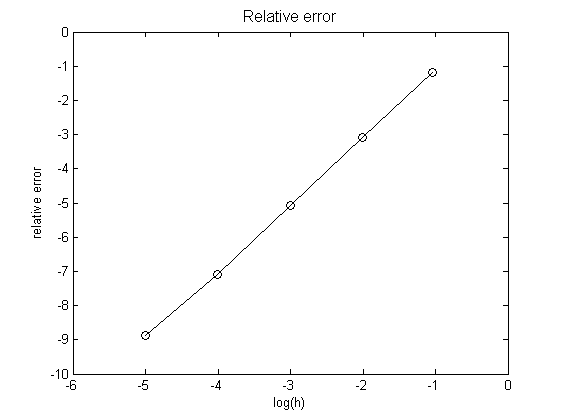
\includegraphics[width=0.75\textwidth]{Figures/relativeerror5.png}
	\caption{Plot of the relative error of the numerical solution to the closed-form solution as a function of the step length. 
	The data point with the greatest relative error is for $n=10$, while the data point for the smallest relative error is for $n=10^5$.
	These data points are connected by a almost straight line with a slope of approximately 2.}
	\label{fig:IntOfResult3}
\end{figure}
In the graph given in \figref{fig:IntOfResult3}, the data points form points on an almost straight line. 
Calculating the slope of the straight line from the $\epsilon_i$ and $\log (h)$ values for $n=10$ and $n=100$ gives
\begin{align}
	\text{slope} = \frac{\Delta \epsilon_i}{\Delta \log (h)}
	= \frac{-3.08804 - (-1.1797)}{-2.00432 - (-1.04139)}
	\approx 1.98 \approx 2
	\label{eq:SlopeOfError}
\end{align}
This is an expected result, since the total error $\epsilon_{total}$ goes as $\mathcal{O}(h^2)$, with $h$ being the step length, due to the two contributions to the total error, namely the approximation error $\epsilon_{approx}$ and the round off error $\epsilon_{ro}$.
Since $\epsilon_{total}$ goes as $\mathcal{O}(h^2)$, the relation between $\epsilon_{i} = \log(\epsilon_{total})$ and $\log (h)$ goes as $\epsilon_{i} = 2\log (h) + \text{constant}$. 

One could, however, imagine that when $n$ is further increased, the round off error will increase, and the linear dependence between $\epsilon_i$ and $\log (h)$ will disappear.
